\documentclass[a4paper,margin=1.54cm]{article}
\usepackage{polski}
\usepackage[utf8]{inputenc}
\usepackage{graphicx}
\usepackage{natbib}
\usepackage{mathtools}
\usepackage{subcaption}
\usepackage{float}
\usepackage{matlab-prettifier}
\usepackage[T1]{fontenc}       % change font encoding to T1

\title{Odwracanie macierzy\\metodą iteracji prostej Jacobiego\\przez rozwiązanie układów równań AX=I\\z macierzą rozrzedzoną A}
\author{Kamil Górzyński\\grupa F1\\Wydział MiNI, Politechnika Warszawska}
%\date{18 października 2018}


\usepackage{blindtext}

\begin{document}

\begin{titlepage}
\maketitle
\end{titlepage}

\section{Wprowadzenie}

\section{Algorytm iteracji prostej Jacobiego\\dla układu równań $Ax = b$ ($x$, $b$ - wektory) }

Niech dana będzie nieosobliwa macierz $A_{n\times n}$ i układ równań liniowych 
$ Ax = b $, \\
którego rozwiązaniem dokładnym jest wektor $x = A^{-1}b$.
\[
A = 
 \begin{bmatrix}
  a_{1,1} & a_{1,2} & \cdots & a_{1,n} \\
  a_{2,1} & a_{2,2} & \cdots & a_{2,n} \\
  \vdots  & \vdots  & \ddots & \vdots  \\
  a_{n,1} & a_{n,2} & \cdots & a_{n,n} 
 \end{bmatrix}
\textrm{,} \quad 
x = 
 \begin{bmatrix}
  x_{1}\\
  x_{2}\\
  \vdots\\
  x_{n}
 \end{bmatrix}
 \textrm{,} \quad 
b = 
 \begin{bmatrix}
  b_{1}\\
  b_{2}\\
  \vdots\\
  b_{n}
 \end{bmatrix}
\]
Wówczas macierz $A$ może zostać zdekomponowana na sumę macierzy diagonalnej $D$, powstałej z wyrazów leżących na diagonali $A$, oraz jej pozostałych elementów, oznaczonych jako macierz $R$: \cite{krupka2009wstep}\cite{stoerwstep} 

\[
A = D + R
\textrm{,} \quad \textrm{gdzie} \quad
D =
 \begin{bmatrix}
  a_{1,1} & 0 & \cdots & 0 \\
  0 & a_{2,2} & \cdots & 0 \\
  \vdots  & \vdots  & \ddots & \vdots  \\
  0 & 0 & \cdots & a_{n,n} 
 \end{bmatrix}
\textrm{,} \quad
R =
 \begin{bmatrix}
  0 & a_{1,2} & \cdots & a_{1,n} \\
  a_{2,1} & 0 & \cdots & a_{2,n} \\
  \vdots  & \vdots  & \ddots & \vdots  \\
  a_{n,1} & a_{n,2} & \cdots & 0
 \end{bmatrix}
\textrm{.}
\]
Zapisując $A$ w postaci zdekomponowanej oraz mnożąc stronami przez $x$, otrzymujemy heurystyczny wzór metody iteracyjnej Jacobiego.
\begin{align*}
A =& D + R\\
Ax =& (D + R)x\\
b =& Dx + Rx\\
Dx =& b - Rx\\
x^{(k+1)} =& D^{-1}(b-Rx^{(k)})\\
x^{(k+1)} =& Tx^{(k)}+C\textrm{,} \quad \textrm{gdzie} \quad T = -D^{-1}R \textrm{,} \quad C=D^{-1}b 
\end{align*}
Za przybliżenie początkowe $x^{(1)}$ przyjmujemy $T\times 0 + C = C$. \\
Przybliżenie końcowe z kolei otrzymamy po odpowiedniej liczbie operacji, kiedy spełniony zostanie warunek zbieżności:
\[
	\|Ax^{(n)} - b\| < d, \quad \textrm{gdzie } d \textrm{ stanowi dopuszczalny błąd residualny.}
\]

\newpage
\section{Zgodność algorytmu z $AX = B$\\($X$, $B$ - macierze kwadratowe)}
W wyprowadzonym powyżej wzorze wektor $x^{(k+1)}_n$ otrzymujemy z sumy iloczynów macierzy $T_{n,n}$, $D^{-1}_{n,n}$ oraz wektorów: $x^{(k)}_n$ i $b_n$.
\[
\begin{bmatrix}
    \qquad\qquad \\
    \\
    \raisebox{0pt}[0pt][0pt]{\Huge $T$} \\
    \\
\end{bmatrix}_{n\times n}
\begin{bmatrix}
 \vdots\\
 x^{(k)}\\
 \vdots
\end{bmatrix}_{n}
\quad + \quad
\begin{bmatrix}
    \qquad\qquad \\
    \\
    \raisebox{0pt}[0pt][0pt]{\Huge $D^{-1}$} \\
    \\
\end{bmatrix}_{n\times n}
\begin{bmatrix}
 \vdots\\
 b\\
 \vdots
\end{bmatrix}_{n}
\quad = \quad
\begin{bmatrix}
 \vdots\\
 x^{(k+1)}\\
 \vdots
\end{bmatrix}_{n}
 \]
 Jest zatem możliwe utworzenie macierzy $X^{(k)}_{n\times n}$ z n wektorów kolumnowych $x^{(k)}_n$ oraz macierzy $B_{n\times n}$ z n wektorów kolumnowych $b_n$. Zastosowanie powyższego wzoru do macierzy utworzonych z n wektorów umożliwia ich jednoczesne przetworzenie.
 \[
 \begin{bmatrix}
    \qquad\qquad \\
    \\
    \raisebox{0pt}[0pt][0pt]{\Huge $T$} \\
    \\
\end{bmatrix}_{n\times n}
 \begin{bmatrix}
    \vdots & & \vdots \\
     x^{(k)}_{i,1} & \cdots & x^{(k)}_{i,n}\\
    \vdots & & \vdots
\end{bmatrix}_{n\times n}
\quad + \quad
\begin{bmatrix}
    \qquad\qquad \\
    \\
    \raisebox{0pt}[0pt][0pt]{\Huge $D^{-1}$} \\
    \\
\end{bmatrix}_{n\times n}
 \begin{bmatrix}
    \vdots & & \vdots \\
     b_{i,1} & \cdots & b_{i,n}\\
    \vdots & & \vdots
\end{bmatrix}_{n\times n}
\quad = 
 \]
\[
=\quad
 \begin{bmatrix}
    \vdots & & \vdots \\
     x^{(k+1)}_{i,1} & \cdots & x^{(k+1)}_{i,n}\\
    \vdots & & \vdots
\end{bmatrix}_{n\times n}
\quad = \quad
\begin{bmatrix}
    \qquad\qquad \\
    \\
    \raisebox{0pt}[0pt][0pt]{\Huge $X^{(k+1)}$} \\
    \\
\end{bmatrix}_{n\times n}
 \]
 
\section{Użycie algorytmu do odwracania macierzy}
Macierz odwrotna $A^{-1}$ to macierz, dla której $A\times A^{-1} = I$.
Umiejąc znajdować rozwiązania układu równań $A\times X = B$, można zauważyć, że dla $B=I$ rozwiązaniem układu równań dla macierzy kwadratowej $A$ jest jej odwrotność. Będziemy zatem wykonywać powyższy algorytm dla:
\[
A\times X = I
\]
Należy przy tym zadbać, aby odwracana była macierz, która spełnia warunek zbieżności metody Jacobiego:
\[
	\|B	\|_\infty < 1, \quad \textrm{gdzie} \quad B = D^{-1}R.
\]
Powyższy warunek jest też spełniony dla każdej macierzy silnie diagonalnie dominującej, czyli wtedy, gdy dla każdego wiersza macierzy $A$ zachodzi:
\[
    \sum_{j=1, i\neq j}^n |a_{i,j}| < |a_{i,i}| \textrm{.}
\]

\newpage

\section{Porównanie działania dla macierzy spełniającej i niespełniającej warunku zbieżności}
% Funkcja pobiera sparse z pliku LFAT5.mat
% Macierz 14x14, 46 elementów niezerowych (ok. 23,5%)
% https://www.cise.ufl.edu/research/sparse/matrices/Oberwolfach/LFAT5.html

Na Rys. \ref{fig:LFAT5}. przedstawiono zbieżność metody Jacobiego zastosowanej do znalezienia odwrotności macierzy LFAT5+189*I (silnie diagonalnie dominującej) oraz macierzy LFAT5, niespełniającej warunku zbieżności.
\begin{figure}[!ht]
    \centering
    %add desired spacing between images, e. g. ~, \quad, \qquad, \hfill etc. 
      %(or a blank line to force the subfigure onto a new line)
    \begin{subfigure}[!ht]{0.45\textwidth}
        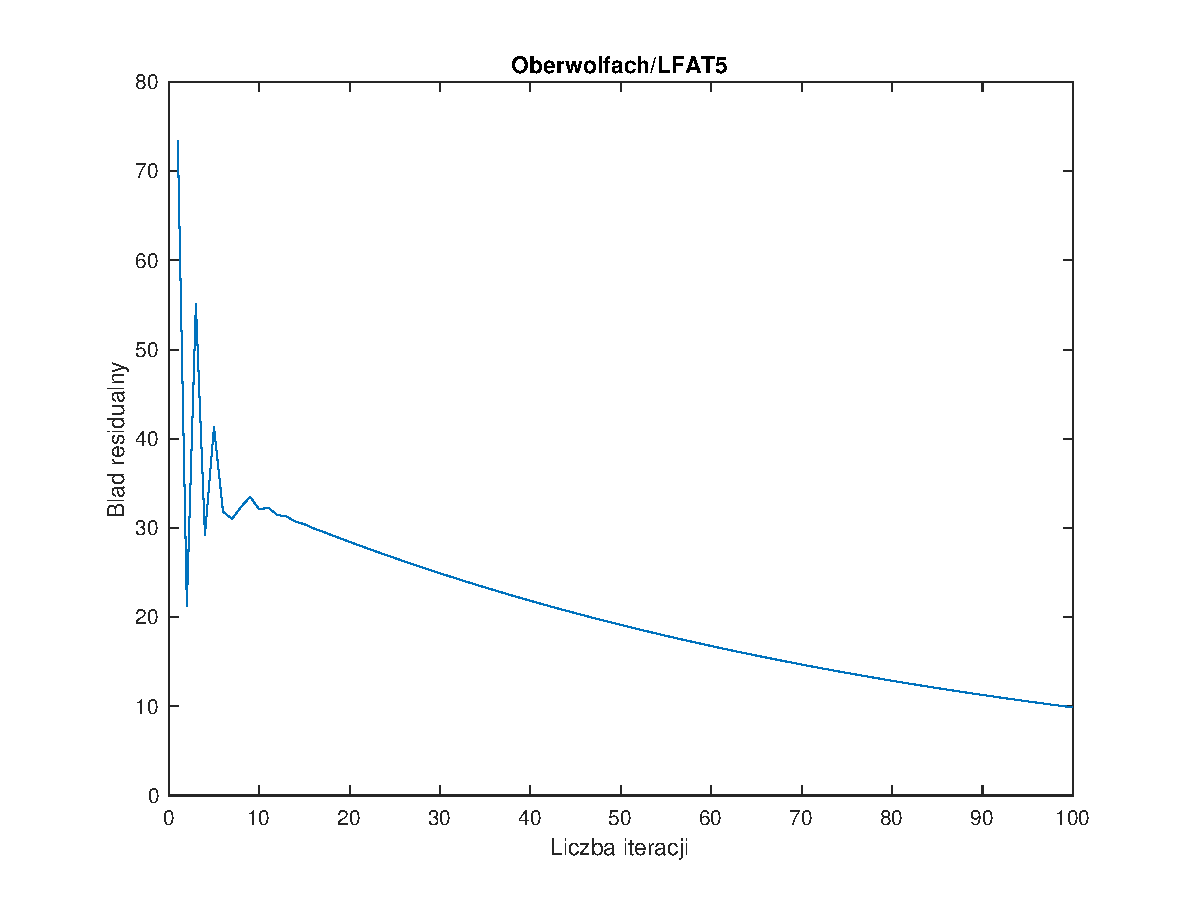
\includegraphics[width=\textwidth]{5niezbiega.eps}
        \caption{Zbieżność dla LFAT5}
        \label{fig:5zbiega}
    \end{subfigure}
    ~ %add desired spacing between images, e. g. ~, \quad, \qquad, \hfill etc. 
    %(or a blank line to force the subfigure onto a new line)
    \begin{subfigure}[!ht]{0.45\textwidth}
        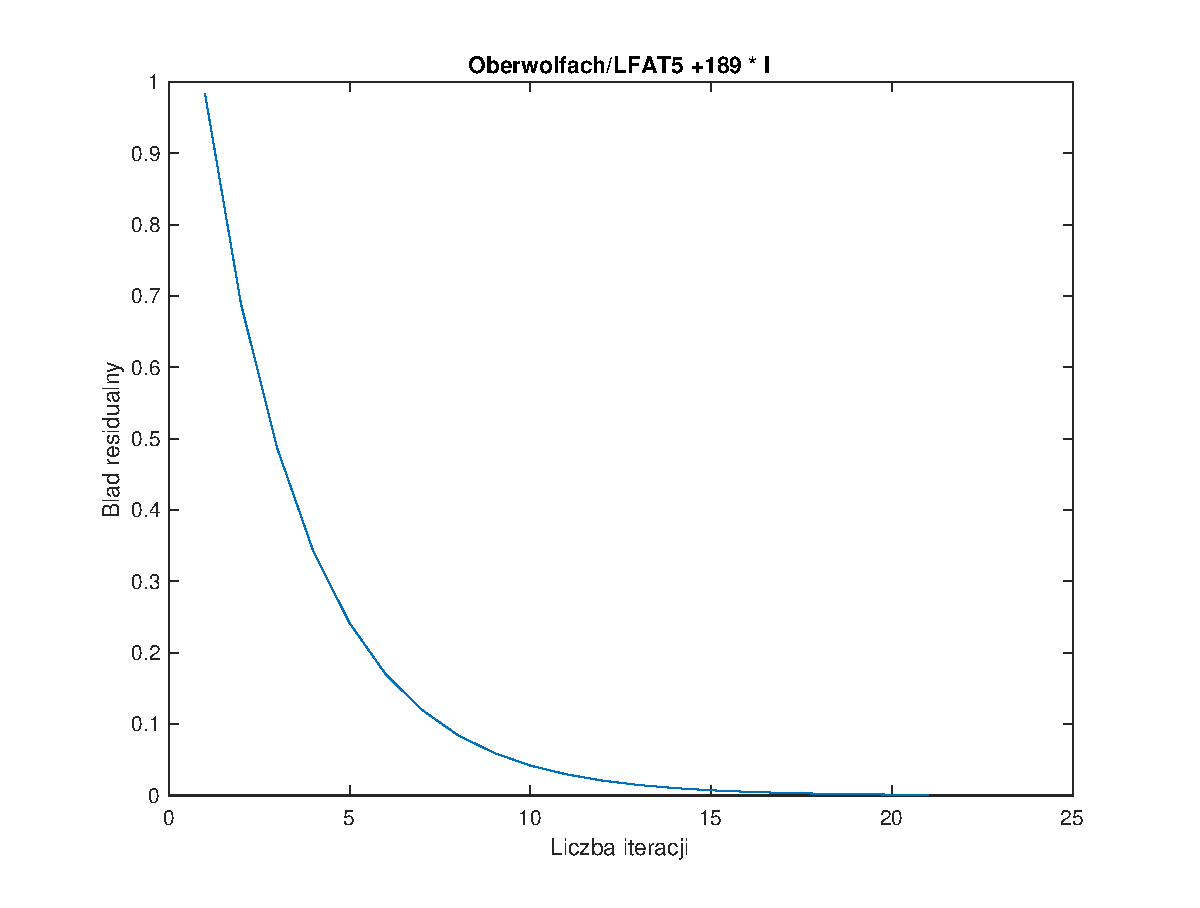
\includegraphics[width=\textwidth]{5zbiega.eps}
        \caption{Zbieżność dla LFAT5+189*I}
        \label{fig:5niezbiega}
    \end{subfigure}
    \caption{Zbieżność metody Jacobiego dla zgodnej i niezgodnej macierzy}\label{fig:LFAT5}
\end{figure}
\\Jak widać na Rys. \ref{fig:LFAT5}, metoda Jacobiego zastosowana do niespełniającej warunku zbieżności macierzy w pierwszych krokach iteracji cechuje się bardzo wysokim błędem, niemalejącym w kolejnych 10 iteracjach. W kolejnych krokach błąd udaje się zmniejszać z każdą następną iteracją, jednak zadowalający błąd na poziomie $\|Ax^{(n)} - b\| < 0,001$ otrzymano dopiero po xxx iteracjach (Rys. \ref{fig:LFAT5}a).\\
Inaczej prezentuje się sytuacja w przypadku macierzy silnie diagonalnie dominującej - po dodaniu $189*I$ do powyższego przykładu, odwróconą macierz z zadowalającym błędem otrzymano już po 21 iteracjach (Rys. \ref{fig:LFAT5}b).\\
W związku z powyższym, aby nie rezygnować z ciekawych do prezentacji przykładów, program posiada funkcję zamieniającą dowolną niezgodną macierz kwadratową na macierz silnie diagonalnie dominującą. 

\begin{lstlisting}[
  style      = Matlab-editor,
  basicstyle = \mlttfamily,
]
function [X, int_coeff] = makedominant(A)
% Uzyskanie macierzy silnie diagonalnie dominujacej poprzez dodanie
% odpowiedniej stalej do kazdej wartosci glownej przekatnej macierzy/sparse

[wynik, mindiff] = czyzbiezna_full_diagdom(A);
int_coeff = ceil(-mindiff);

if(wynik == 1)
    X = A;
    fprintf('Macierz jest juz silnie diagonalnie dominujaca.\n');
else
    X = A + (int_coeff .* speye(size(A)));
    fprintf('Nowa macierz silnie diagonalnie dominujaca: A + %d * I\n', int_coeff);
end
end

\end{lstlisting}

\begin{figure}[!ht]
\centering
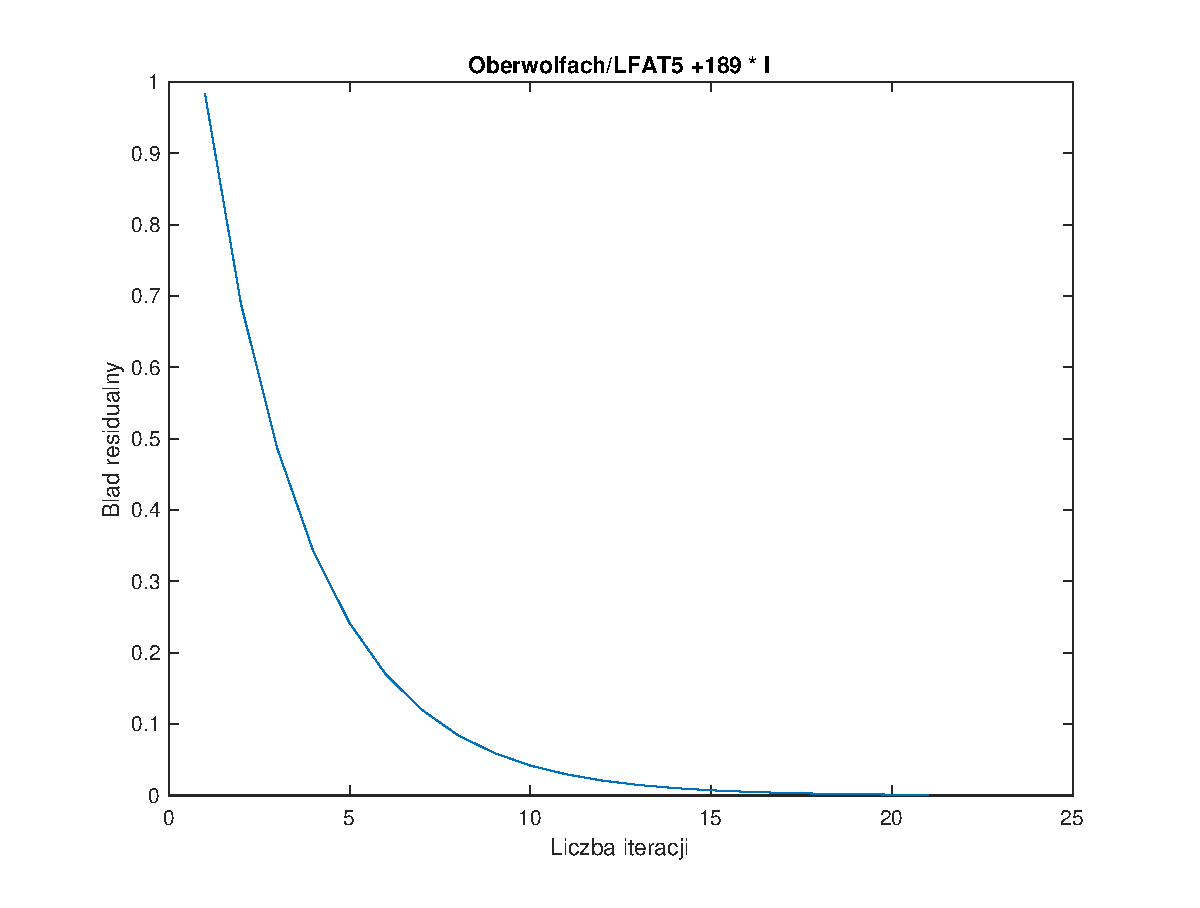
\includegraphics[scale=0.3]{5zbiega.eps}
\caption{Zbieżność metody Jacobiego}
\label{fig:zrzut1}
\end{figure}


\section{Optymalizacja dla macierzy rozrzedzonych}
% Funkcja pobiera sparse z pliku nasa4704.mat
% Macierz 4704x4704, 104756 elementów niezerowych (ok. 0.47%)
% https://www.cise.ufl.edu/research/sparse/matrices/Boeing/nasa4704.html

W przypadku macierzy o dużych rozmiarach, często spotyka się macierze o niskim stopniu wypełnienia (stosunku wyrazów niezerowych do rozmiaru macierzy), zwane macierzami rozrzedzonymi (ang. \textit{sparse matrices}). W przypadku przetwarzania macierzy rozrzedzonej wprowadza się optymalizację, polegającą na zapisie jedynie elementów różnych od zera. W ten sposób zmniejszamy zarówno wymagania pamięciowe, jak i liczbę operacji zmiennoprzecinkowych potrzebnych do prowadzenia działań na macierzy (np. w przypadku mnożenia macierzy przez wektor, nie będziemy mnożyć przez zera!)\cite{mimuwprzykre}.

\begin{lstlisting}[
  style      = Matlab-editor,
  basicstyle = \mlttfamily,
]
%% Code sections are highlighted.
% System command are supported...
!touch testFile.txt
A = [1, 2, 3;... %... as is line continuation.
     4, 5, 6];
fid = fopen('testFile.text', 'w');
for k=1:10
  fprintf(fid, '%6.2f \n', k)
end
x=1; %% this is just a comment, not the start of a section
% Context-sensitive keywords get highlighted correctly...
p = properties(person); %(here, properties is a function)
x = linspace(0,1,101);
y = x(end:-1:1);
% ... even in nonsensical code.
]end()()(((end while {    end    )end ))))end (end
%{
    block comments are supported
%} even
runaway block comments
are
\end{lstlisting}

\section{Introduction}
There is a theory which states that if ever anyone discovers exactly what the Universe is for and why it is here, it will instantly disappear and be replaced by something even more bizarre and inexplicable.
There is another theory which states that this has already happened.

\begin{figure}[!ht]
\centering
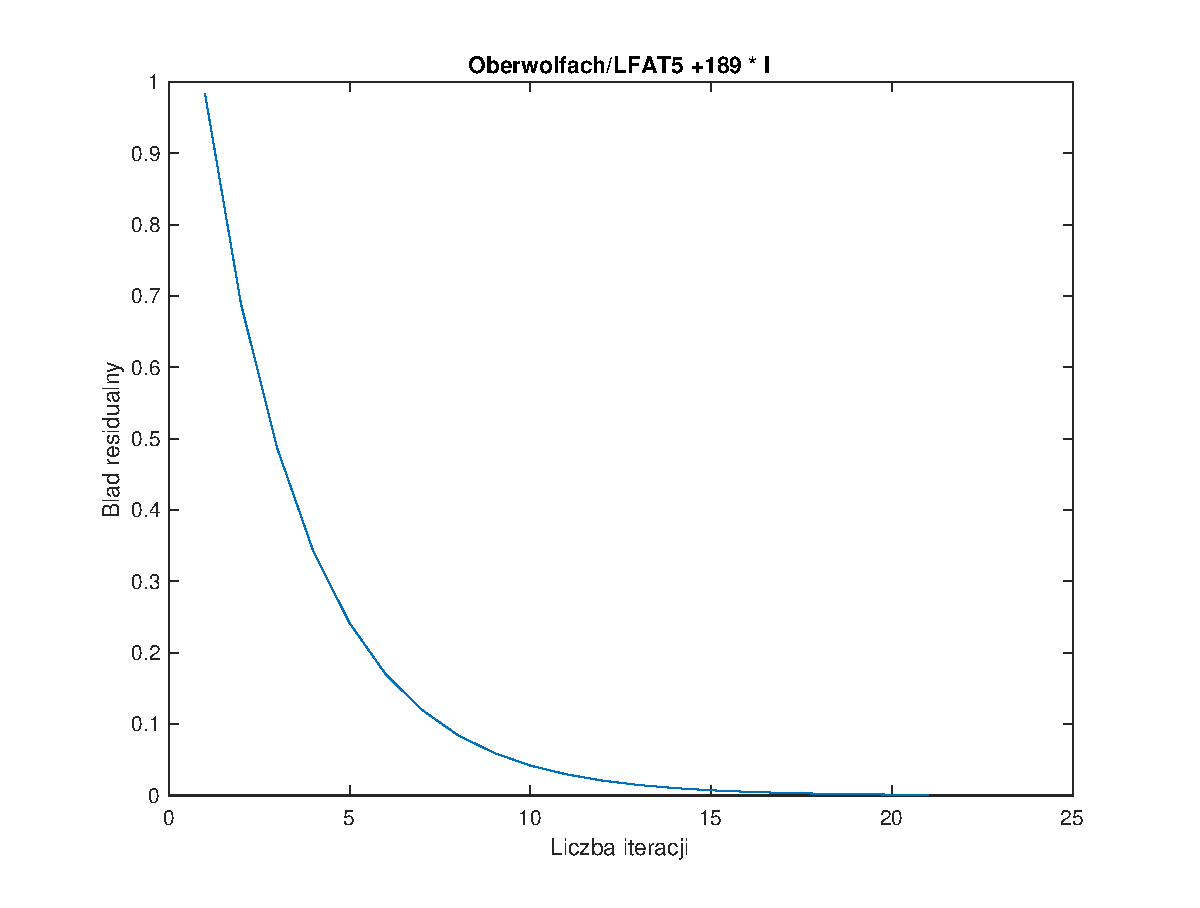
\includegraphics[scale=0.3]{5zbiega.eps}
\caption{Zbieżność metody Jacobiego}
\label{fig:zrzut2}
\end{figure}

\begin{figure}[!ht]
\centering
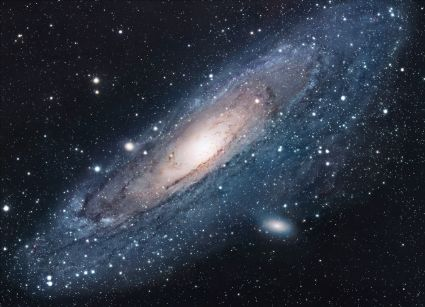
\includegraphics[width=\textwidth]{universe}
\caption{The Universe}
\label{fig:universe}
\end{figure}

\section{Podsumowanie}
Jak wynika z obliczeń, metoda Jacobiego w przypadku odwracania macierzy rozrzedzonych jest znacznie bardziej efektywna zarówno czasowo, jak i pamięciowo, kiedy wykonujemy ją na macierzach typu \textit{sparse} niż na tradycyjnych tablicach. Nie zmienia to jednak faktu, że duże macierze, występujące w fizycznych zastosowaniach, często nie spełniają warunku zbieżności metody. Powoduje to, że dobrą zbieżność uzyskuje się jedynie przy odwracaniu określonej grupy macierzy. 

\bibliographystyle{plain}
\bibliography{references}
\end{document}
